\section{Layer Merger Experiments}
\label{sec:layer_merger}
%% ============================================================

\subsection{Motivation}

A key empirical finding from \S\ref{sec:probes} (shown in Fig.~\ref{fig:consecutive_layer_sim}) is that
EGPT attention outputs exhibit substantially higher consecutive-layer cosine similarity than
standard GPT: $0.176$ vs.\ $0.119$ (adjacent pairs), rising to $\sim 0.53$ for the middle
layers 8--9 of a 12-layer V1 EGPT.  This suggests that EGPT layers may be doing
\emph{redundant} work --- a prerequisite for structural compression via layer merging.
Ideally one could (i) train a 12-layer EGPT and then collapse it to 6 layers at near-zero
cost, recovering most of the original performance.

However, initial naive experiments (averaging adjacent weight pairs, no fine-tuning)
showed that the post-merge perplexity is too high to be useful, despite the high activation
cosine similarity.  The discrepancy suggests that functional similarity in activation space
does not automatically transfer to structural mergability in weight space: adjacent layers
may apply \emph{similar} transformations but be \emph{calibrated} differently (e.g.\ with
opposite signs on certain sub-spaces, or rotated representations).

We pursue three complementary strategies to close this gap.

%% -----------------------------------
\subsection{Strategy A: Cosine-Similarity Regularisation During Training}
\label{sec:cosreg}
%% -----------------------------------

\paragraph{Method.}
\textbf{V39/V40 (activation cosreg):}
We add a differentiable cosine-similarity term to the training objective:
\begin{equation}
  \mathcal{L}_{\mathrm{cos}} = \lambda \sum_{(i,j)\in\mathcal{P}}
      \bigl(\cos\!\operatorname{sim}(\mathbf{a}_i, \mathbf{a}_j) - 1\bigr)^2 ,
\end{equation}
where $\mathbf{a}_i\in\mathbb{R}^{B\cdot T\times D}$ is the attention output of energy block $i$,
$\lambda$ is the regularisation coefficient, and $\mathcal{P}$ contains pairs
$(i,i{+}1)$, $(i,i{+}2)$, $(i,i{+}4)$.
This is an \emph{activation}-based regulariser — it pushes adjacent layers to produce
similar output patterns on the training distribution, but does not directly align weight matrices.

\textbf{V48 (per-matrix weight cosreg):}
The more natural regulariser for enabling weight merging penalises directly the cosine distance
between corresponding weight matrices:
\begin{equation}
  \mathcal{L}_{\mathrm{wcos}} = \frac{\lambda}{|\mathcal{P}|} \sum_{(i,j)\in\mathcal{P}}
      \sum_{W \in \{W_Q, W_K, W_V, W_O, W_1, W_2, W_\mathrm{proj}\}}
      \bigl(1 - \cos\!\operatorname{sim}(\mathrm{vec}(W^{(i)}), \mathrm{vec}(W^{(j)}))\bigr) ,
\end{equation}
where $\mathrm{vec}(\cdot)$ flattens each matrix individually.
The sum is over \emph{individual} weight matrices rather than a single concatenated vector ---
this ensures each matrix (e.g.\ $W_Q$, $W_K$, $W_\mathrm{proj}$) is aligned separately,
preventing large matrices from dominating the cosine similarity of the concatenated vector.
For sandwich architectures, the regularisation applies only to EGPT block pairs; GPT blocks
are excluded (their weight matrices serve a different functional role and should not be
pulled toward the EGPT weight manifold).

\paragraph{Runs.}
\begin{itemize}
  \item \textbf{V39} (176M, $\lambda{=}0.01$, $k{=}10$): EGPT 12$\times$1, $d{=}768$, lr=2e-3.
        Identical to V1 except for the regulariser.  30k steps.
  \item \textbf{V40} (400M, $\lambda{=}0.01$, $k{=}10$): EGPT 24$\times$1, $d{=}1024$, lr=7e-4.
        Identical to the 400M V1 except for the regulariser.  30k steps.
  \item \textbf{V48} (176M, $\lambda{=}0.01$, per-matrix weight cosreg):
        EGPT 12$\times$1, $d{=}768$, lr=2e-3.  30k steps.  Regularises weight matrices
        rather than activations.
  \item \textbf{V50} (400M, $\lambda{=}0.01$, per-matrix weight cosreg):
        EGPT 24$\times$1, $d{=}1024$, lr=7e-4.  30k steps (in progress at 15k).
  \item \textbf{V52} (176M, $\lambda{=}0.1$, $k{=}10$): 10$\times$ stronger constant activation cosreg.
        Tests whether V39's negligible alignment change was simply due to insufficient regularisation strength.
  \item \textbf{V53} (176M, $\lambda$ ramped $0{\to}1.0$ over 30k steps, cosine schedule):
        $\lambda(t) = \bigl(1 - \cos(\pi t / T)\bigr)/2$ where $T{=}30\,000$.
        Motivation: early training benefits from free exploration of the loss landscape;
        the ramp progressively forces alignment only after the model has settled near
        a basin, nudging it towards an \emph{aligned} minimum without disrupting
        initial representation learning.
\end{itemize}

\paragraph{Expected outcomes.}
If $\lambda$ is too large the regulariser will dominate the LM loss and degrade PPL.
If too small it will have negligible effect.  The target regime is: slightly higher
consecutive cosine similarity compared to V1, with $\leq$0.5~PPL points degradation,
and noticeably better post-merge (collapsed-layer) PPL when we apply the merger.

\paragraph{Results.}
Figure~\ref{fig:cosreg_perf} and Table~\ref{tab:cosreg_benchmarks} summarise
the performance impact.

\textbf{Training loss.}
At 176M scale: V39 (act-cosreg) achieves loss 3.273 ($+$0.002 vs V1=3.271); V48 (wt-cosreg)
achieves 3.287 ($+$0.016 vs V1).  Both regularisers impose only marginal cost on perplexity
at $\lambda{=}0.01$.  At 400M scale: V40 (act-cosreg) reached loss $\approx$3.22 at step 15900
(training resumed); V50 (wt-cosreg) reached 3.259 at step 15000 (training in progress).

\textbf{Downstream benchmarks (176M).}
We evaluated V0 GPT, V1 EGPT, and V39 act-cosreg on 8 standard tasks (ARC-c/e, BoolQ, COPA,
HellaSwag, MMLU, WinoGrande, PIQA).
The cosreg has negligible downstream impact: V39 average accuracy 0.463 vs V1 0.458
(both substantially below V0 GPT 0.476).
Per-task differences are within noise ($<$0.02 on every task).
V48 benchmark evaluation is pending (eval job submitted Apr 25).

\textbf{Layer alignment.}
Activation-space analysis (Apr 25, 2026) shows V39 successive
cosine similarity mean = 0.922, essentially identical to V1 (0.939).
The regulariser \emph{did} increase attn sub-output similarity slightly (AttnAvg:
0.339 vs V1 0.296), but the effect on overall block-output similarity was negligible.

\textbf{Summary.}
At 176M scale, V39 act-cosreg ($\lambda{=}0.01$) imposes essentially no
penalty (10-task avg 46.3\% vs V1 46.5\% and V0 46.7\%); the weight-cosreg
V48 loses 1.6 points (44.9\%). Stronger activation cosreg costs more:
V52 ($\lambda{=}0.1$) drops to 45.7\% ($-$0.8 vs V1) and V53 (cosine ramp
$0{\to}1.0$) to 45.4\% ($-$1.1) — see Table~\ref{tab:cosreg_benchmarks} and
Fig.~\ref{fig:bar_cosreg_benchmarks}. Per-task: V52 wins ARC-C (25.3) and
PIQA (63.7); among EGPT variants V53 is best on ARC-E (45.4). All numbers
use \texttt{acc\_norm} where defined by harness convention, matching the
headline tables.
Alignment-vs-accuracy: light cosreg is free; stronger cosreg trades a small
accuracy hit for what we expect to be measurably higher inter-layer alignment
(full heatmaps pending cluster run 20260426). V40/V50 400M results are
pending completion.

\begin{table}[h]
\centering
\caption{Cosreg benchmark accuracies — 176M scale (30k steps).
Avg is the 10-task mean (ARC-c/e, BoolQ, COPA, HellaSwag, MMLU, ObQA, PIQA,
SciQ, WinoGrande). Auto-generated by \texttt{make\_tables.py}.}
\label{tab:cosreg_benchmarks}
\resizebox{\textwidth}{!}{%
% Auto-generated by experiments/energy-inference/scripts/multi-block-ablation/make_tables.py
% Table: cosreg_benchmarks
% DO NOT edit by hand — re-run the generator instead.
\begin{tabular}{lrrrrrrrr}
\toprule
\textbf{Model} & \textbf{Avg$\uparrow$} & \textbf{ARC-c} & \textbf{ARC-e} & \textbf{BoolQ} & \textbf{HellaS} & \textbf{MMLU} & \textbf{PIQA} & \textbf{Wino.} \\
\midrule
V0 GPT 12$\times$1 & 47.5\% & 20.1 & \textbf{51.6} & 56.6 & \textbf{29.6} & \textbf{25.2} & \underline{64.0} & \textbf{51.7} \\
V1 EGPT 12$\times$1 & \underline{47.6\%} & 18.4 & 47.9 & \textbf{61.1} & 28.5 & 23.5 & 62.6 & 50.7 \\
V39 act-cosreg & \textbf{47.7\%} & 20.1 & 49.1 & 58.2 & 28.5 & 23.9 & 63.2 & 50.7 \\
V48 wt-cosreg & 46.2\% & 18.7 & 45.0 & \underline{58.6} & 27.5 & 24.3 & 61.1 & 50.4 \\
V52 act-cosreg $\lambda{=}0.1$ & 46.9\% & \underline{20.3} & 48.7 & 56.6 & 28.6 & 24.4 & \textbf{64.1} & 51.7 \\
V53 act-cosreg ramp$\to$1.0 & 46.6\% & \textbf{21.2} & \underline{50.0} & 53.0 & \underline{28.7} & \underline{24.6} & 62.8 & 49.7 \\
\bottomrule
\end{tabular}
}
\end{table}

\begin{figure}[h]
\centering
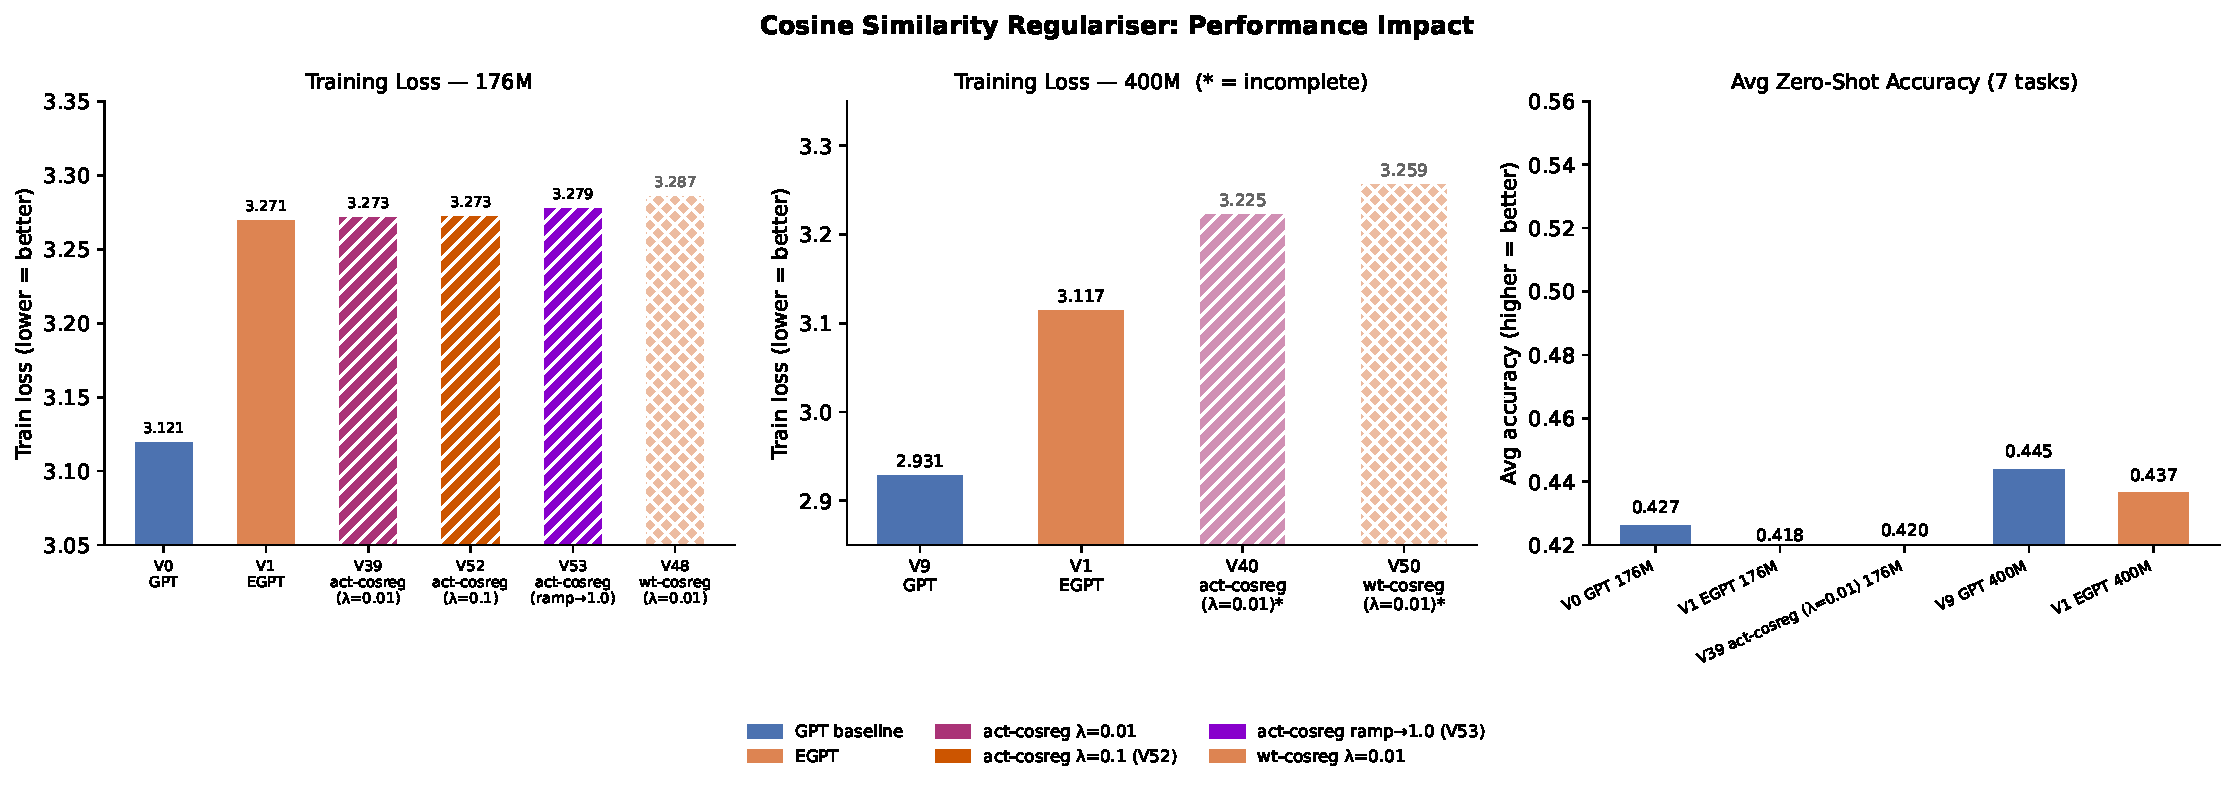
\includegraphics[width=\textwidth]{../results/multi-block-ablation/plots/cosreg_performance_comparison.pdf}
\caption{Cosine similarity regulariser performance comparison.
\emph{Left:} Training loss at 176M scale.  \emph{Centre:} Training loss at 400M scale
(faded bars = training incomplete).  \emph{Right:} Average zero-shot accuracy on 7 tasks
for models with completed evaluations.
The regulariser ($\lambda{=}0.01$) imposes minimal loss overhead ($<$0.02 at 176M) and
negligible downstream accuracy degradation, validating it as a safe pretraining objective.
}
\label{fig:cosreg_perf}
\end{figure}

%% -----------------------------------
\subsection{Strategy B: Post-Training Layer Merger with Fine-Tuning}
\label{sec:merge_finetune}
%% -----------------------------------

\paragraph{Method.}
Starting from the fully trained V1 EGPT 12-layer checkpoint, we merge adjacent pairs
$(0{+}1), (2{+}3), \ldots, (10{+}11)$ into a 6-layer model, then fine-tune for 5k steps
at lr=2e-4 (10$\times$ lower than the scratch LR).  We compare two merge strategies:

\textbf{Naive merge (V42)}: average all corresponding tensors element-wise:
$\tilde{W} = (W_i + W_j)/2$.

\textbf{Procrustes-aligned merge (V43)}: for each 2D weight matrix, find the orthogonal
rotation $R$ minimising $\|W_i - W_j R\|_F$ via SVD
$(U, S, V^\top) = W_i^\top W_j \Rightarrow R = VU^\top$,
then set $\tilde{W} = (W_i + W_j R)/2$.  The alignment corrects for any arbitrary
rotation symmetry between the two layers before averaging, reducing the destructive
interference that plagues naive averaging.

The merged model is saved as a standalone HF checkpoint and loaded by the fine-tune
config as a pre-trained initialisation.

\paragraph{Runs.}
\begin{itemize}
  \item \textbf{V42}: Naive merge of V1 $\to$ 6 layers (6$\times$1, half compute), fine-tuned 5k steps.
  \item \textbf{V43}: Procrustes-aligned merge of V1 $\to$ 6 layers (6$\times$1), fine-tuned 5k steps.
  \item \textbf{V44}: Naive merge of V1 $\to$ 6 unique blocks with \texttt{layer\_iterations}$=[2]^6$
        (6$\times$2, iso-compute), fine-tuned 5k steps.
  \item \textbf{V45}: Procrustes-aligned merge $\to$ 6$\times$2 iso-compute, fine-tuned 5k steps.
\end{itemize}
Note: V42/V43 inadvertently halved compute by setting \texttt{layer\_iterations}$=[1]^6$.
V44/V45 correct this by summing iterations across each merged pair, preserving total depth.

\paragraph{Baseline.}
The 12-layer V1 achieves train loss 3.271 at 30k steps.
A 6$\times$1 EGPT trained from scratch would be expected to converge around 3.4--3.5.

\paragraph{Results.}
\begin{itemize}
  \item \textbf{V42 naive init}: activation cosine sim = 0.644 (very disrupted);
        after 5k FT: loss = 3.691, activation cos-sim = 0.855.
  \item \textbf{V43 Procrustes init}: activation cos-sim = 0.756 (better start);
        after 5k FT: loss = 3.640, activation cos-sim = 0.853.
  \item \textbf{V44 naive 6$\times$2 (iso-compute)}: fine-tuned 5k steps at lr=2e-4 (cosine).
        Final loss = 3.606.
  \item \textbf{V45 Procrustes 6$\times$2 (iso-compute)}: fine-tuned 5k steps at lr=2e-4.
        Final loss = 3.584.
\end{itemize}
Procrustes alignment provides a meaningfully better initialisation (0.756 vs 0.644)
and reaches lower final loss consistently.
The iso-compute V44/V45 improve over V42/V43 (+0.08 loss units) but remain far from
the V1 baseline (3.271), a gap of $>0.3$ nats.

\begin{figure}[h]
\centering
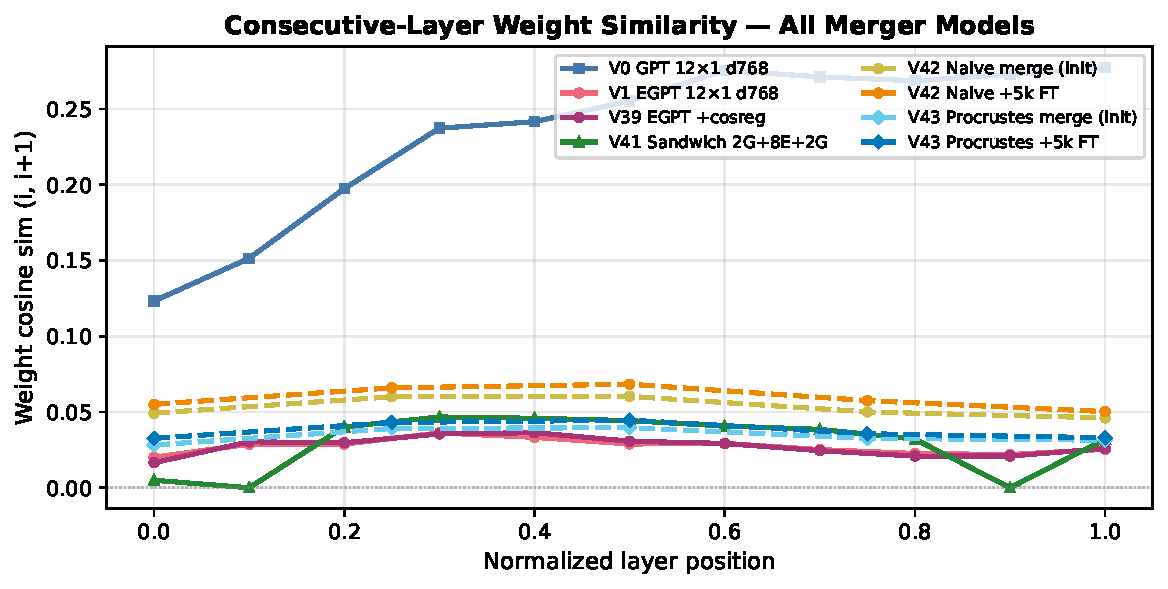
\includegraphics[width=\textwidth]{../results/multi-block-ablation/plots/merger_successive_cosim_all.pdf}
\caption{Successive-pair residual-stream cosine similarity by layer position for all merger variants
  (V0 GPT, V1 EGPT, V39+cosreg, V42 naive, V43 Procrustes: init and after 5k FT).
  Procrustes initialisation raises pre-FT similarity throughout; fine-tuning drives all 6-layer
  models toward the V1 EGPT curve despite the different architecture depth.}
\label{fig:merger_successive}
\end{figure}

\begin{figure}[h]
\centering
\begin{minipage}[t]{0.48\textwidth}
  \centering
  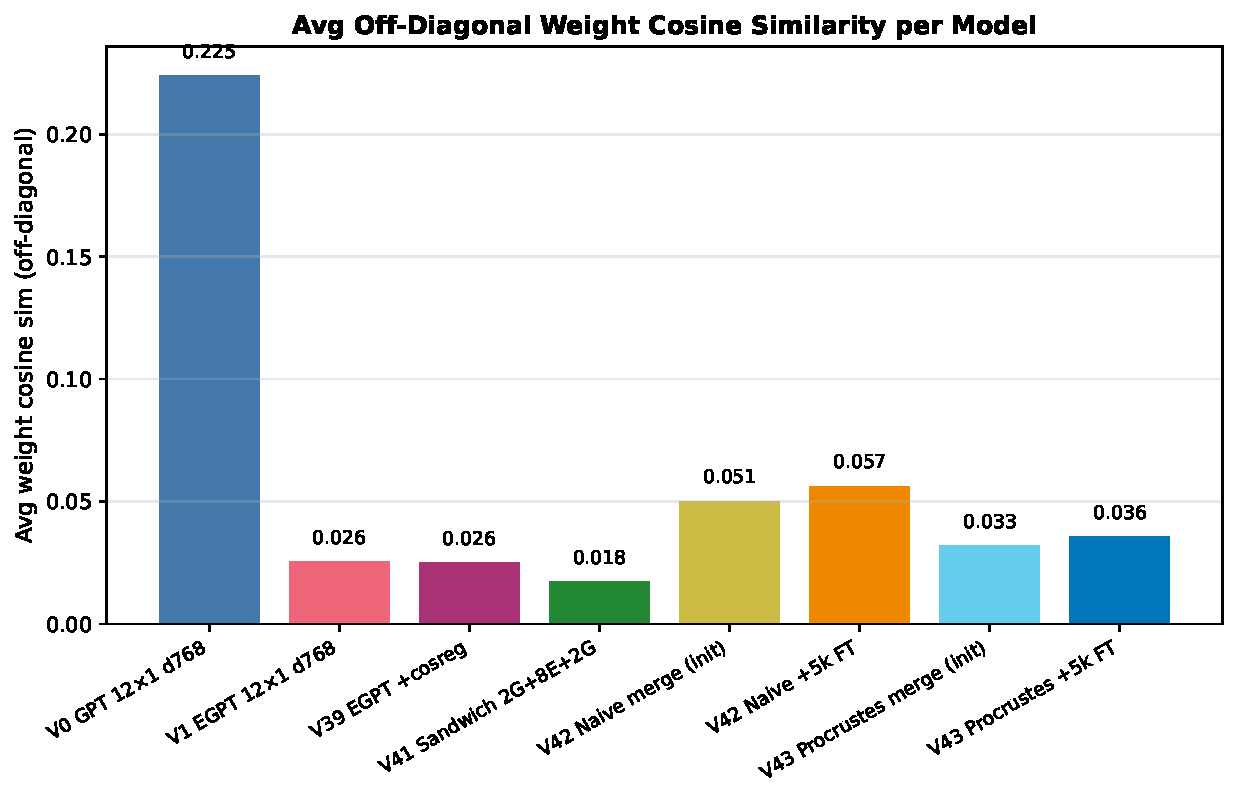
\includegraphics[width=\textwidth]{../results/multi-block-ablation/plots/merger_avg_cosim_bar.pdf}
  \caption{Off-diagonal mean weight cosine similarity per model.}
  \label{fig:merger_avg_bar}
\end{minipage}\hfill
\begin{minipage}[t]{0.48\textwidth}
  \centering
  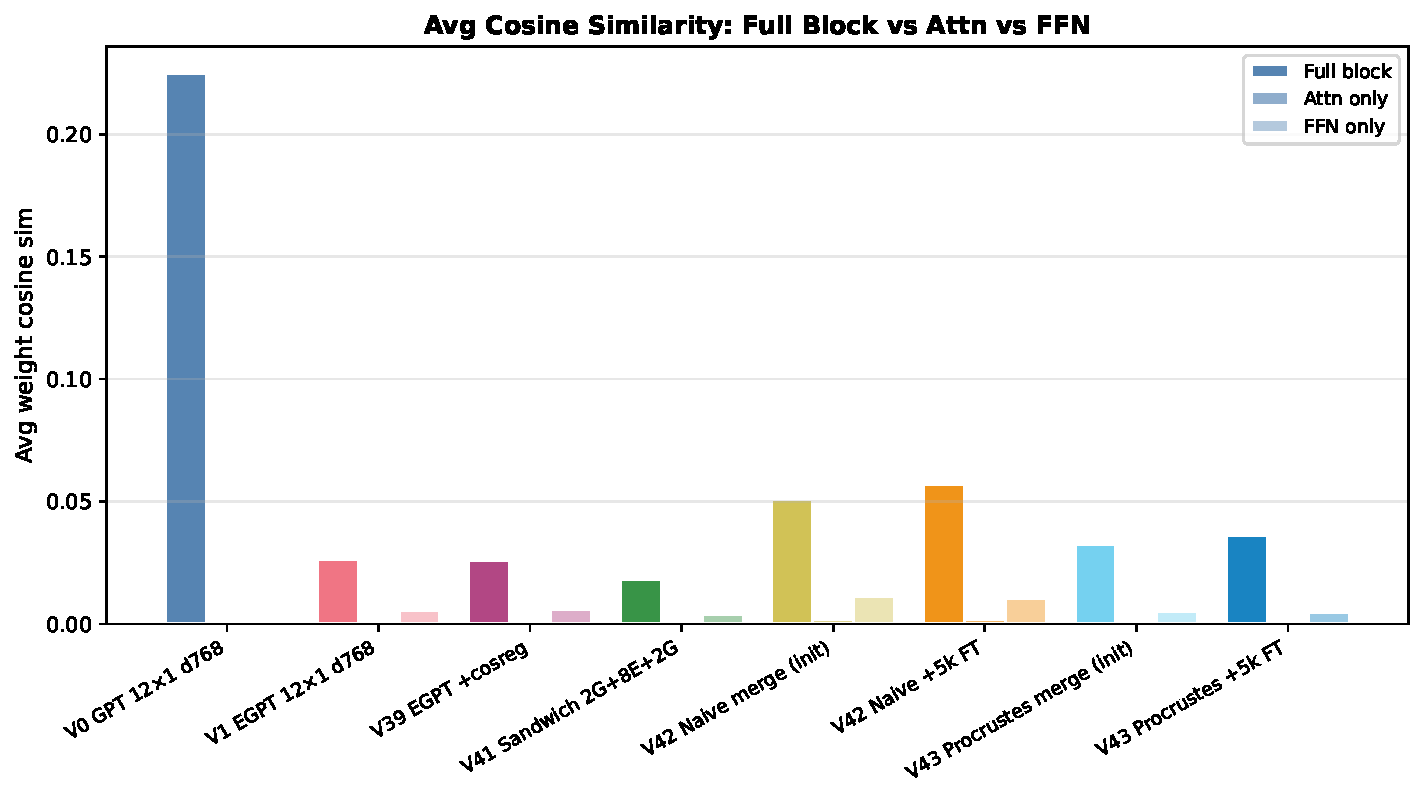
\includegraphics[width=\textwidth]{../results/multi-block-ablation/plots/merger_avg_cosim_attn_ffn_bar.pdf}
  \caption{Attn vs.\ FFN breakdown of off-diagonal mean cosine similarity.}
  \label{fig:merger_avg_attn_ffn}
\end{minipage}
\end{figure}

\begin{figure}[h]
\centering
\begin{minipage}[t]{0.48\textwidth}
  \centering
  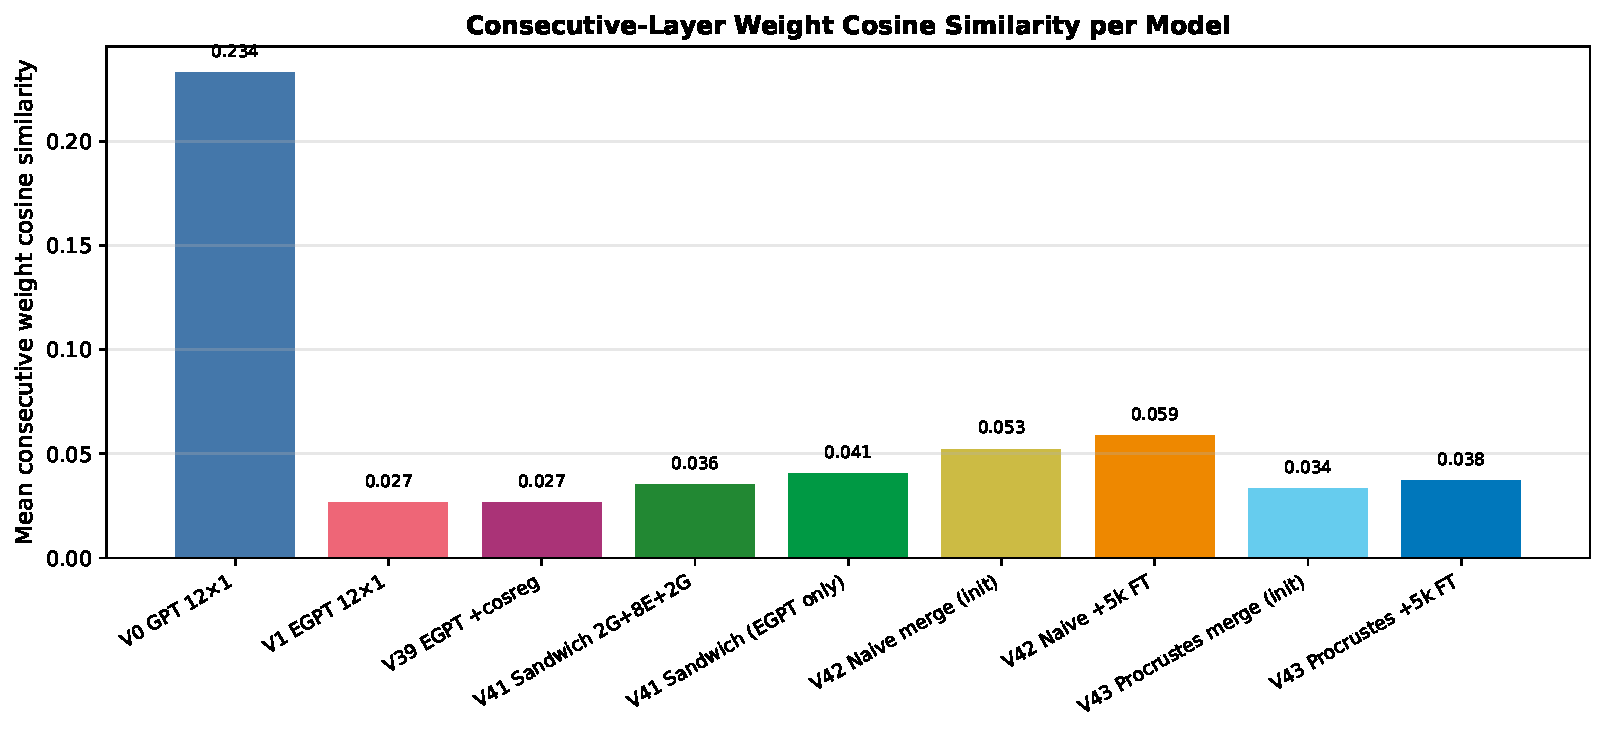
\includegraphics[width=\textwidth]{../results/multi-block-ablation/plots/merger_consec_avg_cosim_bar.pdf}
  \caption{Consecutive-layer mean weight cosine similarity (adjacent pairs). Includes V41 EGPT-only entry.}
  \label{fig:merger_consec_bar}
\end{minipage}\hfill
\begin{minipage}[t]{0.48\textwidth}
  \centering
  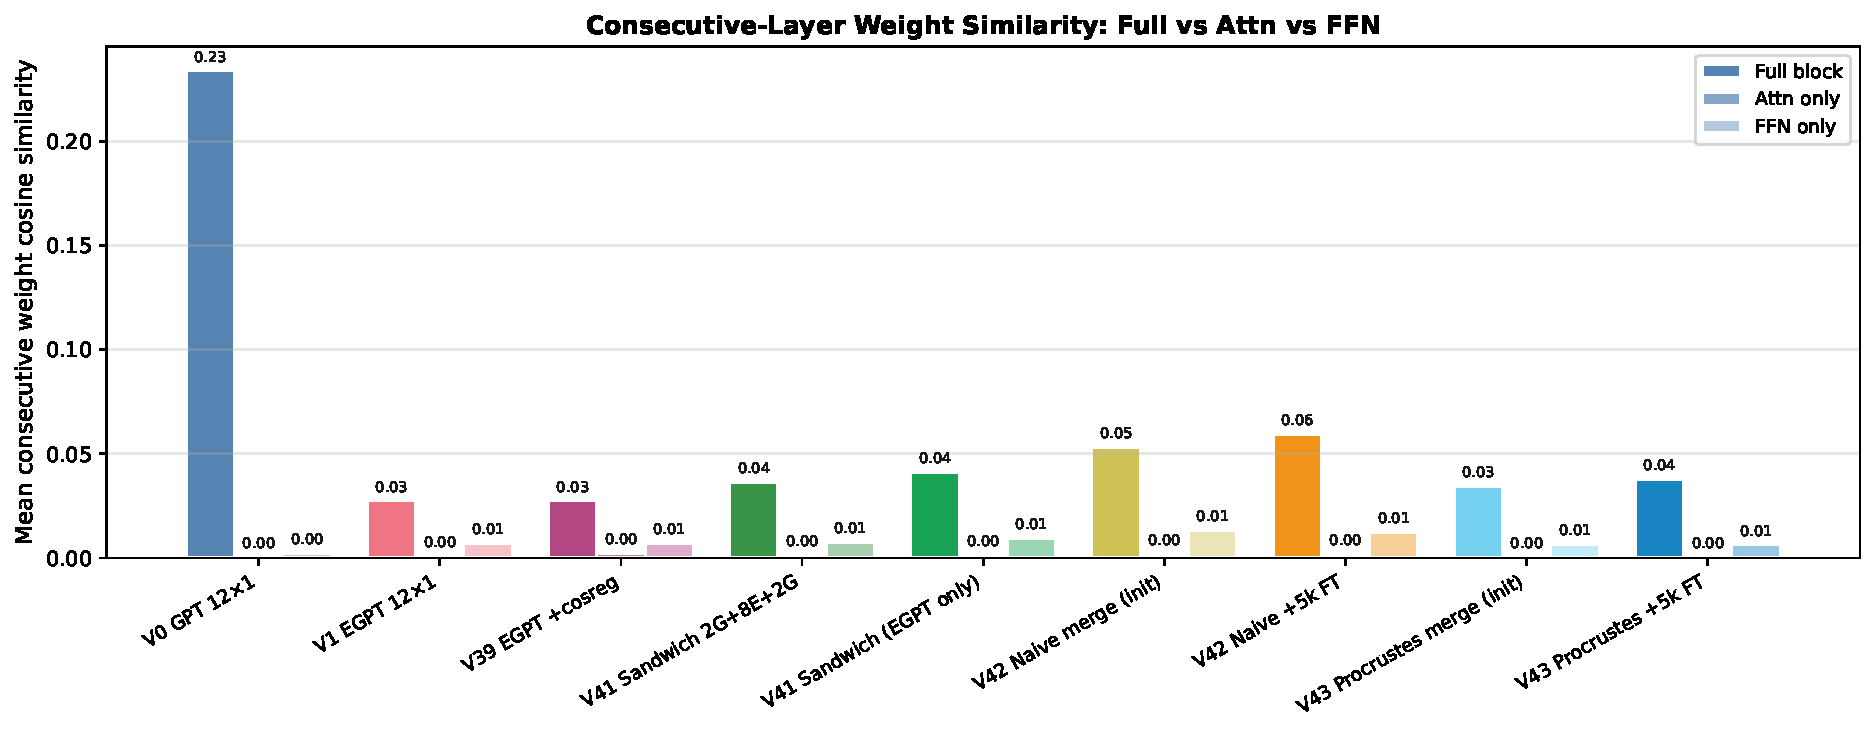
\includegraphics[width=\textwidth]{../results/multi-block-ablation/plots/merger_consec_avg_cosim_attn_ffn_bar.pdf}
  \caption{Consecutive-layer Attn vs.\ FFN weight cosine similarity breakdown. V41 EGPT-only isolates EGPT-EGPT pairs.}
  \label{fig:merger_consec_attn_ffn}
\end{minipage}
\end{figure}

A plausible cause: by step 5k the cosine LR schedule decays to $0.1\times$ the peak,
leaving lr $= 2\times 10^{-5}$ --- a factor of 100$\times$ below the original training LR.
The model may still be in an early recovery phase at that point, and the very low LR
prevents further progress.  We are testing this hypothesis with:
\begin{itemize}
  \item \textbf{V46}: Procrustes 6$\times$2 init, \emph{constant} lr=2e-4 (no decay), 5k steps.
  \item \textbf{V47}: Procrustes 6$\times$2 init, cosine from lr=2e-3 (original V1 training LR, 10$\times$ higher), 5k steps.
\end{itemize}

\paragraph{Activation-space layer similarity.}
We use three metrics to probe layer similarity, each measuring a different thing:
\begin{enumerate}
  \item \textbf{Residual-stream cosine} $\cos(h_\mathrm{out}^{(i)},\, h_\mathrm{out}^{(i+1)})$:
        highly confounded by the passthrough residual; random baseline $\approx 0.87$.
  \item \textbf{Sequential-delta cosine} $\cos(\Delta_i, \Delta_{i+1})$ where $\Delta_i = h_\mathrm{out}^{(i)} - h_\mathrm{in}^{(i)}$:
        unconfounded from passthrough but confounded by the evolving input distribution
        (each block receives a different input in the forward pass).
  \item \textbf{Same-input delta cosine} $\cos(\Delta_i^*, \Delta_{i+1}^*)$ where
        $\Delta_i^* = \mathrm{Block}_i(h) - h$ for the \emph{same fixed} base embedding $h$
        fed to every block independently:
        the cleanest measure of \emph{functional similarity} between operators.
\end{enumerate}

\begin{table}[h]
\centering
\caption{Activation similarity under all three metrics (successive-pair means).
  ``Rand'' = same-input delta for an untrained random model (near zero by construction).
  $\|\Delta\|/\|h\|$ = mean block update magnitude relative to residual stream norm.}
\label{tab:act_sim_full}
\small
\begin{tabular}{lcrrrr}
\toprule
\textbf{Model} & \textbf{N} & \textbf{Resid.} & \textbf{Seq.$\Delta$} & \textbf{Same$\Delta$} & $\|\Delta\|/\|h\|$ \\
\midrule
V0 GPT 12$\times$1         & 12 & 0.904 & 0.322 & 0.100 & 1.18 \\
V1 EGPT 12$\times$1        & 12 & 0.939 & 0.074 & \textbf{0.536} & 7.94 \\
V39 EGPT+cosreg            & 12 & 0.922 & 0.100 & 0.529 & 7.07 \\
V41 Sandwich 2G+8E+2G      & 12 & 0.889 & 0.116 & 0.370 & 2.72 \\
\midrule
V42 Naive merge (init)     &  6 & 0.644 & $-$0.262 & 0.398 & 5.15 \\
V42 Naive $+$5k FT         &  6 & 0.855 & 0.027 & 0.261 & 5.04 \\
V43 Procrustes merge (init) & 6 & 0.756 & $-$0.120 & 0.430 & 6.88 \\
V43 Procrustes $+$5k FT    &  6 & 0.853 & 0.022 & 0.395 & 8.51 \\
\midrule
Random (V1 arch)           & 12 & 0.870 & --- & $-$0.005 & --- \\
\bottomrule
\end{tabular}
\end{table}

\begin{figure}[h]
\centering
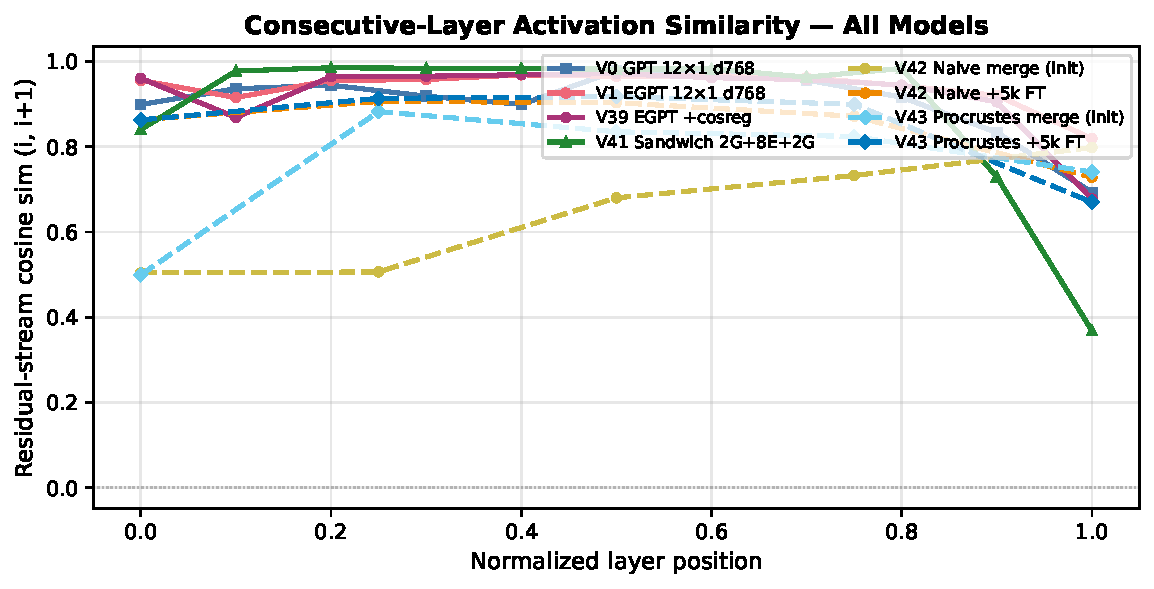
\includegraphics[width=\textwidth]{../results/multi-block-ablation/plots/act_successive_cosim_all.pdf}
\caption{Successive-pair same-input delta cosine similarity by layer position (all models).
  V1 EGPT inner layers form a high-similarity plateau; merger initialisation disrupts it;
  fine-tuning partially restores structure but at lower values than V1.}
\label{fig:act_successive}
\end{figure}

\begin{figure}[h]
\centering
\begin{minipage}[t]{0.48\textwidth}
  \centering
  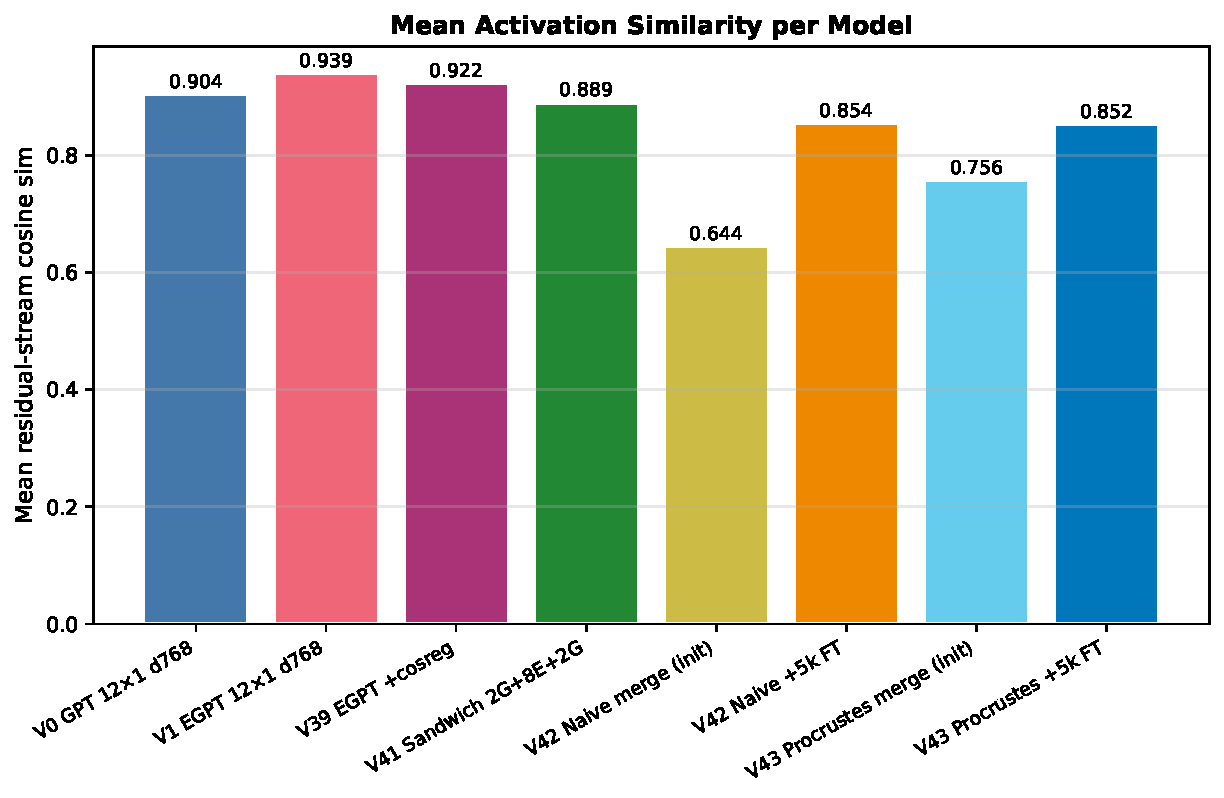
\includegraphics[width=\textwidth]{../results/multi-block-ablation/plots/act_avg_cosim_bar.pdf}
  \caption{Consecutive-layer mean residual-stream cosine similarity per model (already consecutive, not off-diagonal).}
  \label{fig:act_avg_bar}
\end{minipage}\hfill
\begin{minipage}[t]{0.48\textwidth}
  \centering
  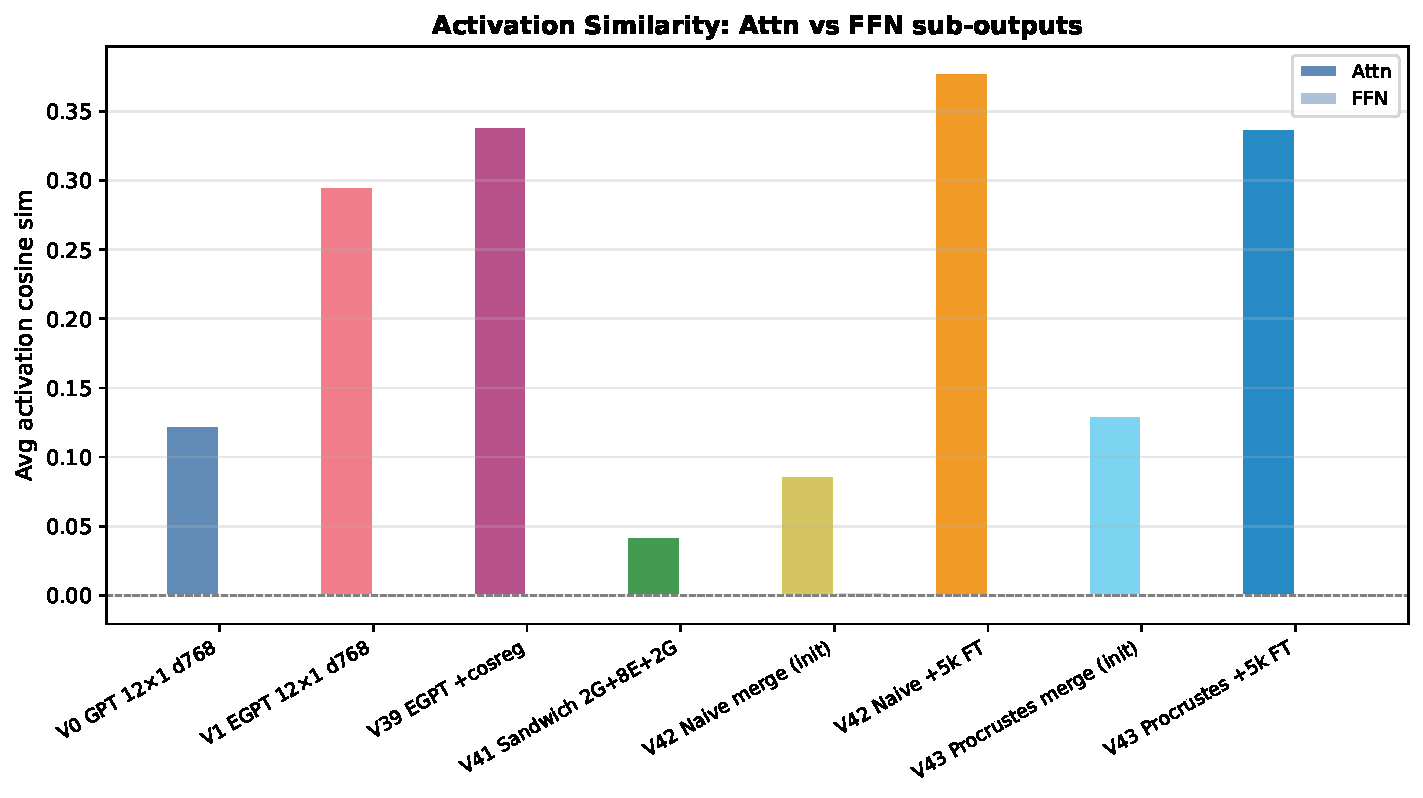
\includegraphics[width=\textwidth]{../results/multi-block-ablation/plots/act_avg_cosim_attn_ffn_bar.pdf}
  \caption{Attn vs.\ FFN breakdown of off-diagonal mean activation cosine similarity.}
  \label{fig:act_avg_attn_ffn}
\end{minipage}
\end{figure}

\begin{figure}[h]
\centering
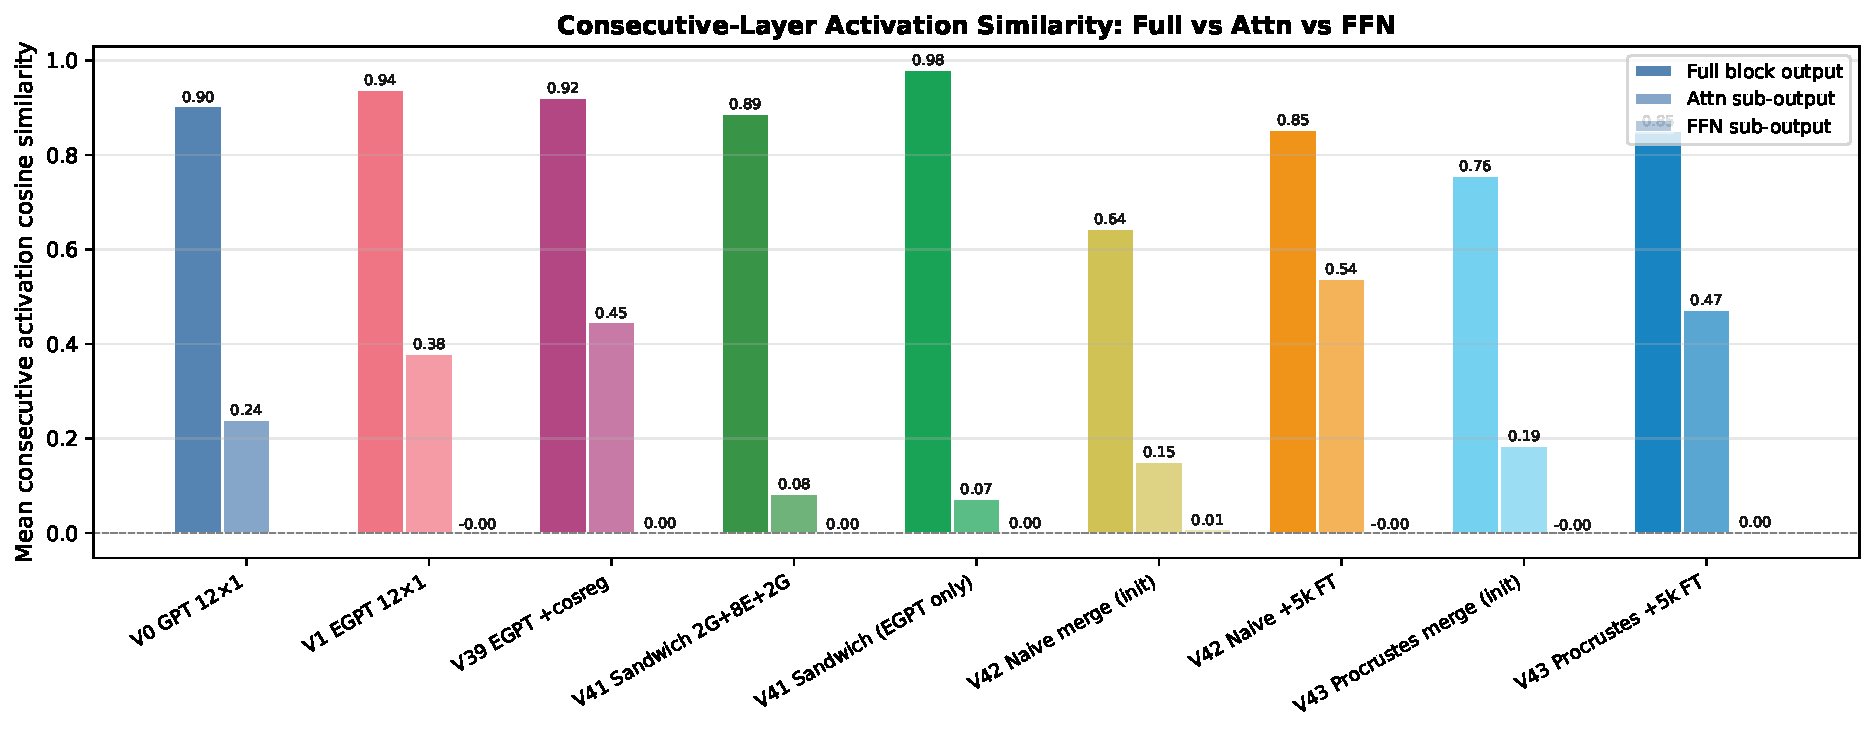
\includegraphics[width=\textwidth]{../results/multi-block-ablation/plots/act_consec_avg_cosim_attn_ffn_bar.pdf}
\caption{Consecutive-layer activation cosine similarity breakdown: residual stream, attn sub-output, FFN sub-output.
  V41 EGPT-only entry shows consecutive similarity for EGPT-EGPT layer pairs only.}
\label{fig:act_consec_attn_ffn}
\end{figure}

Key findings from the same-input delta metric (Table~\ref{tab:act_sim_full}):
\begin{itemize}
  \item \textbf{EGPT blocks are functionally highly redundant (0.536 vs GPT 0.100).}
        Given the same base embedding $h$, adjacent EGPT blocks compute strongly correlated
        updates.  GPT layers specialize: each layer applies a distinct transformation.
        This is the strongest evidence to date that EGPT layers could in principle be merged.

  \item \textbf{The residual-stream metric (0.939) is nearly fully explained by the random baseline
        (0.870).} The real signal comes from same-input delta; residual-stream similarity
        is inflated by the passthrough connection and should not be used as a mergeability proxy.

  \item \textbf{Fine-tuning after merge reduces functional similarity} (V42: $0.398 \to 0.261$;
        V43: $0.430 \to 0.395$). The 6 merged blocks \emph{differentiate} during recovery ---
        they specialize to handle the very different inputs they see at each position in the
        forward pass.  This is the correct behaviour for a deep model, but it means naive
        merge+FT does not converge back to the EGPT redundancy regime.

  \item \textbf{EGPT blocks make large updates} ($\|\Delta\|/\|h\| \approx 7.9$) vs GPT ($1.2$).
        Even though EGPT blocks apply correlated update \emph{directions}, the updates are
        large, causing the sequential residual stream to drift far from $h$ after each step.
        This is the key reason why the sequential-delta metric is near-zero for EGPT (blocks
        see very different inputs) while same-input delta is high (the operator itself is similar).

  \item \textbf{V41 EGPT core layers show the highest pairwise similarity (0.78--0.87)},
        while boundary GPT layers have near-zero same-input delta similarity (0.04--0.21).
        Within the 8-block EGPT core, pairs (3,4), (4,5), (5,6) reach 0.839, 0.869, 0.780;
        only the last EGPT block (just before the output GPT layers) breaks the pattern ($-0.052$),
        suggesting it serves as a projection-back operator rather than a pure gradient step.

  \item \textbf{EGPT functional redundancy is not in the attn or FFN sub-outputs individually.}
        Breaking the same-input delta into sub-components (Table~\ref{tab:act_sim_breakdown}).
        Each value below is the cosine similarity \emph{between} delta vectors of adjacent blocks:
        $\cos(\Delta_i^*, \Delta_{i+1}^*)$ where $\Delta_i^* = \mathrm{sub\text{-}output}_i(h)$.
        \begin{itemize}
          \item Attn sub-output: $\cos(\Delta^\mathrm{attn}_i, \Delta^\mathrm{attn}_{i+1}) = 0.198$ (moderate; well above random 0.001).
          \item FFN sub-output: $\cos(\Delta^\mathrm{ffn}_i, \Delta^\mathrm{ffn}_{i+1}) = 0.001$ (essentially random).
          \item Full-block output: $\cos(\Delta^\mathrm{full}_i, \Delta^\mathrm{full}_{i+1}) = \mathbf{0.536}$ (much higher than either sub-component).
        \end{itemize}
        The redundancy emerges from the \emph{projection layer} ($W_\mathrm{proj}$) combining
        attn and FFN outputs: the \texttt{dual\_unconstrained} projection (separate $W_\mathrm{proj\_attn}$
        and $W_\mathrm{proj\_mlp}$) learns to apply a correlated linear map across blocks even
        from decorrelated sub-components.
        GPT attn sub-outputs also show moderate alignment (0.153) --- higher than the full-block
        metric (0.100), because the MLP adds block-specific diversity that lowers the full-block
        similarity below the attn-alone level.
        The V41 Sandwich EGPT core shows the opposite pattern: high full-block $\delta$ (0.84--0.87 for
        inner pairs) but very low attn sub-output $\delta$ (0.022 overall), suggesting GPT boundary layers
        pre-process the input into a stable representation that makes the projection weights align
        strongly across EGPT blocks.
\end{itemize}

\begin{table}[h]
\centering
\caption{Successive-pair cosine similarity of same-input delta vectors:
  $\mathrm{cos}(\Delta_i^*, \Delta_{i+1}^*)$ where $\Delta_i^* = \mathrm{Block}_i(h)-h$
  for the same base embedding $h$.
  ``Full'' = full-block $\Delta$; ``Attn'' / ``FFN'' = raw sub-outputs before projection;
  ``proj(Attn)'' = $\mathrm{proj\_attn}(a_i)$ for \texttt{dual\_unconstrained} blocks;
  ``proj(FFN)'' = $\mathrm{proj\_mlp}(f_i)$.
  All values are \emph{cosine similarities between deltas}, not delta magnitudes.
  EGPT's high full-block alignment (0.536) despite low raw attn (0.198) and near-zero FFN (0.001)
  implies the projection layer is the source of inter-block alignment.
  ``proj(Attn)'' and ``proj(FFN)'' columns isolate exactly which stream the proj amplifies.}
\label{tab:act_sim_breakdown}
\small
\begin{tabular}{lrrrrrrr}
\toprule
\textbf{Model} & \textbf{Loss} & \textbf{N} & $\cos(\Delta^\mathrm{full})$ & $\cos(\Delta^\mathrm{attn})$ & $\cos(\mathrm{proj(attn)})$ & $\cos(\Delta^\mathrm{ffn})$ & $\cos(\mathrm{proj(FFN)})$ \\
\midrule
V0 GPT 12$\times$1         & 3.271 & 12 & 0.100 & 0.153 & ---  & --- & --- \\
V1 EGPT 12$\times$1        & 3.271 & 12 & 0.536 & 0.198 & 0.034 & 0.001 & \textbf{0.496} \\
V39 EGPT+act-cosreg        & 3.273 & 12 & 0.529 & 0.212 & 0.021 & 0.000 & 0.490 \\
V41 Sandwich 2G+8E+2G      & 3.403 & 12 & 0.370 & 0.022 & 0.078$^\dagger$ & 0.000 & 0.526$^\dagger$ \\
\midrule
V42 Naive $+$5k FT         & ---   &  6 & 0.261 & 0.234 & 0.047 & $-$0.003 & 0.228 \\
V43 Procrustes $+$5k FT    & ---   &  6 & 0.395 & 0.146 & 0.019 & $-$0.002 & 0.332 \\
Random baseline            & ---   & 12 & $-$0.002 & --- & --- & --- & --- \\
\bottomrule
\end{tabular}
\smallskip

\noindent\small$^\dagger$V41 Sandwich: proj columns computed over the 8 EGPT blocks only (positions 2--9);
GPT boundary blocks have no \texttt{proj\_attn}/\texttt{proj\_mlp}.
\end{table}

\begin{figure}[h]
\centering
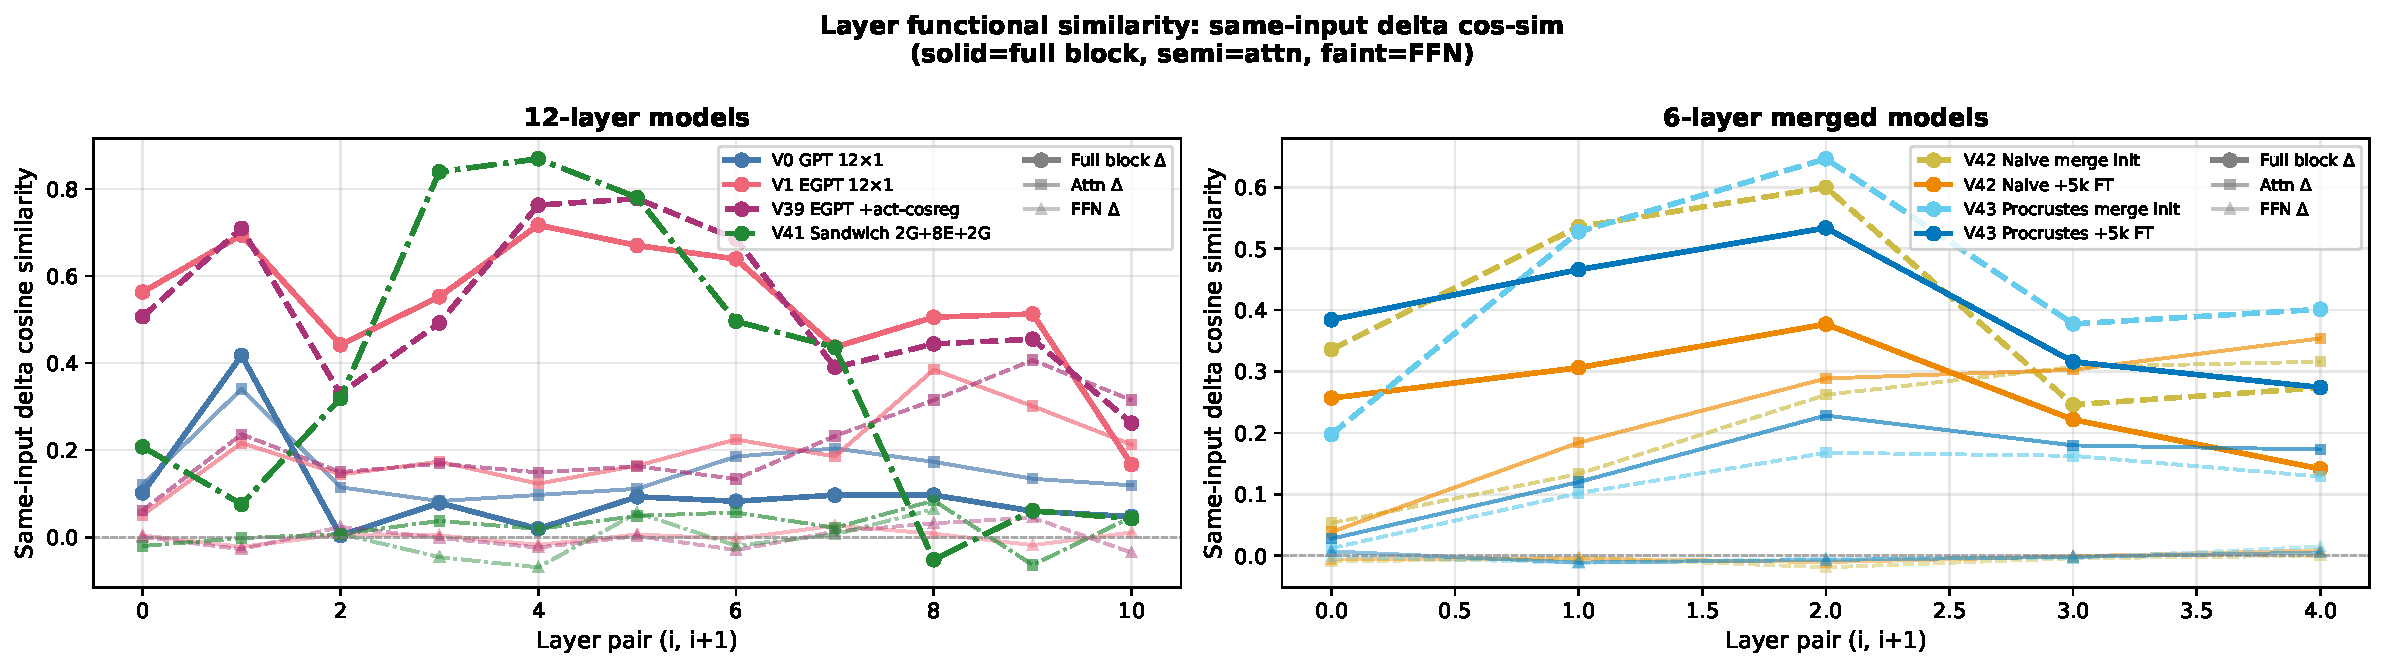
\includegraphics[width=\textwidth]{../results/multi-block-ablation/plots/same_delta_successive_full_attn_ffn.pdf}
\caption{Same-input delta cosine similarity by layer pair, decomposed into full-block (solid, thick),
  attn sub-output (semi-transparent), and FFN sub-output (faint).
  EGPT's high full-block similarity (0.536) is not explained by attn (0.198) or FFN (0.001) alone ---
  it emerges from the projection layer combining them.}
\label{fig:same_delta_successive}
\end{figure}

\begin{figure}[h]
\centering
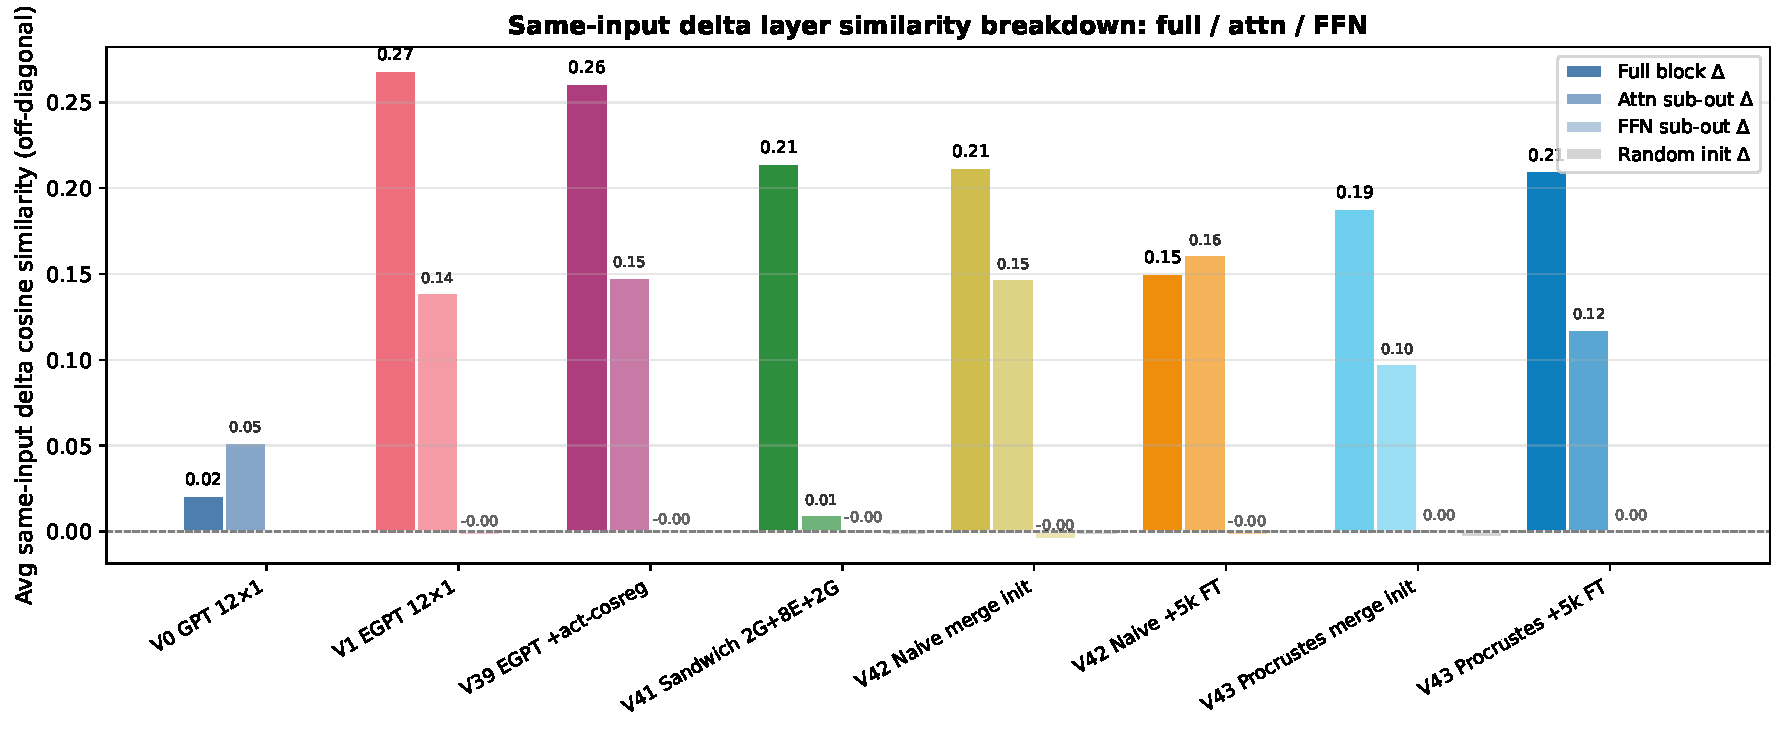
\includegraphics[width=\textwidth]{../results/multi-block-ablation/plots/same_delta_breakdown_bar.pdf}
\caption{Average \emph{off-diagonal} same-input delta cosine similarity: full block vs.\ attn sub-output
  vs.\ FFN sub-output vs.\ random-init baseline.}
\label{fig:same_delta_breakdown}
\end{figure}

\begin{figure}[h]
\centering
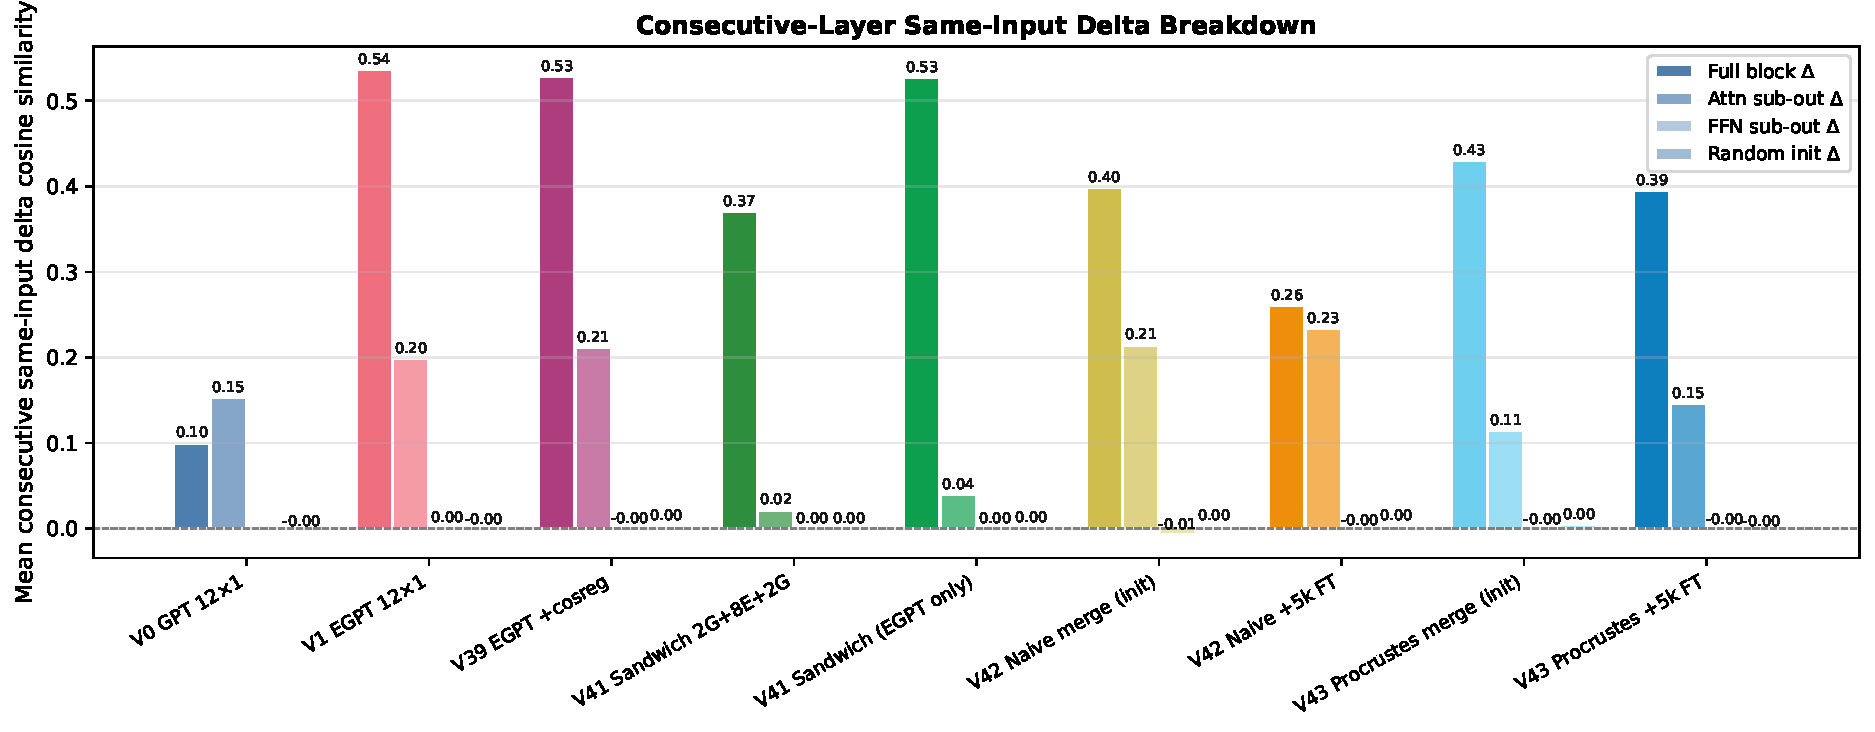
\includegraphics[width=\textwidth]{../results/multi-block-ablation/plots/same_delta_consec_breakdown_bar.pdf}
\caption{Average \emph{consecutive-layer} same-input delta cosine similarity: full block vs.\ attn
  vs.\ FFN vs.\ random baseline. V41 EGPT-only entry uses only EGPT-EGPT adjacent pairs.}
\label{fig:same_delta_consec_breakdown}
\end{figure}

\paragraph{Projection decomposition: \texttt{proj\_mlp} is the source of all inter-block alignment.}
For \texttt{dual\_unconstrained} blocks, $\Delta_i = -\mathrm{proj\_attn}_i(a_i) - \mathrm{proj\_mlp}_i(f_i)$.
Analysis of the projected contributions (Table~\ref{tab:act_sim_breakdown}, Figure~\ref{fig:proj_decomp_successive}) reveals a striking result:

\begin{itemize}
  \item \textbf{\texttt{proj\_mlp} creates alignment from noise.}
    Raw FFN outputs are near-random across blocks ($\approx$0.001), yet
    $\mathrm{cos}(\mathrm{proj\_mlp}_i(f_i),\, \mathrm{proj\_mlp}_{i+1}(f_{i+1})) = 0.496$ ---
    nearly as large as the full-block delta (0.536).
    The \texttt{proj\_mlp} matrices are sufficiently similar across blocks that they map
    orthogonal FFN inputs to consistently aligned output directions.

  \item \textbf{\texttt{proj\_attn} destroys alignment.}
    Raw attn outputs have moderate alignment (0.198), but after
    \texttt{proj\_attn}: $\mathrm{cos}(\mathrm{proj\_attn}_i(a_i),\, \mathrm{proj\_attn}_{i+1}(a_{i+1})) = 0.034$.
    The per-block learned attn projection matrices are \emph{not} similar across blocks,
    and actually suppress the moderate inter-block alignment of attention outputs.

  \item \textbf{Conclusion:} EGPT's high full-block alignment comes almost entirely from
    \texttt{proj\_mlp}, not attention.  The same pattern holds for V39 (act-cosreg) and
    V41 Sandwich, suggesting this is a structural property of \texttt{dual\_unconstrained}
    training, not an artifact of any specific regulariser.
    This directly motivates weight cosreg (V48/V50): if \texttt{proj\_mlp} weight similarity
    drives functional alignment, training to maximise that similarity should improve mergeability.
\end{itemize}

\begin{figure}[h]
\centering
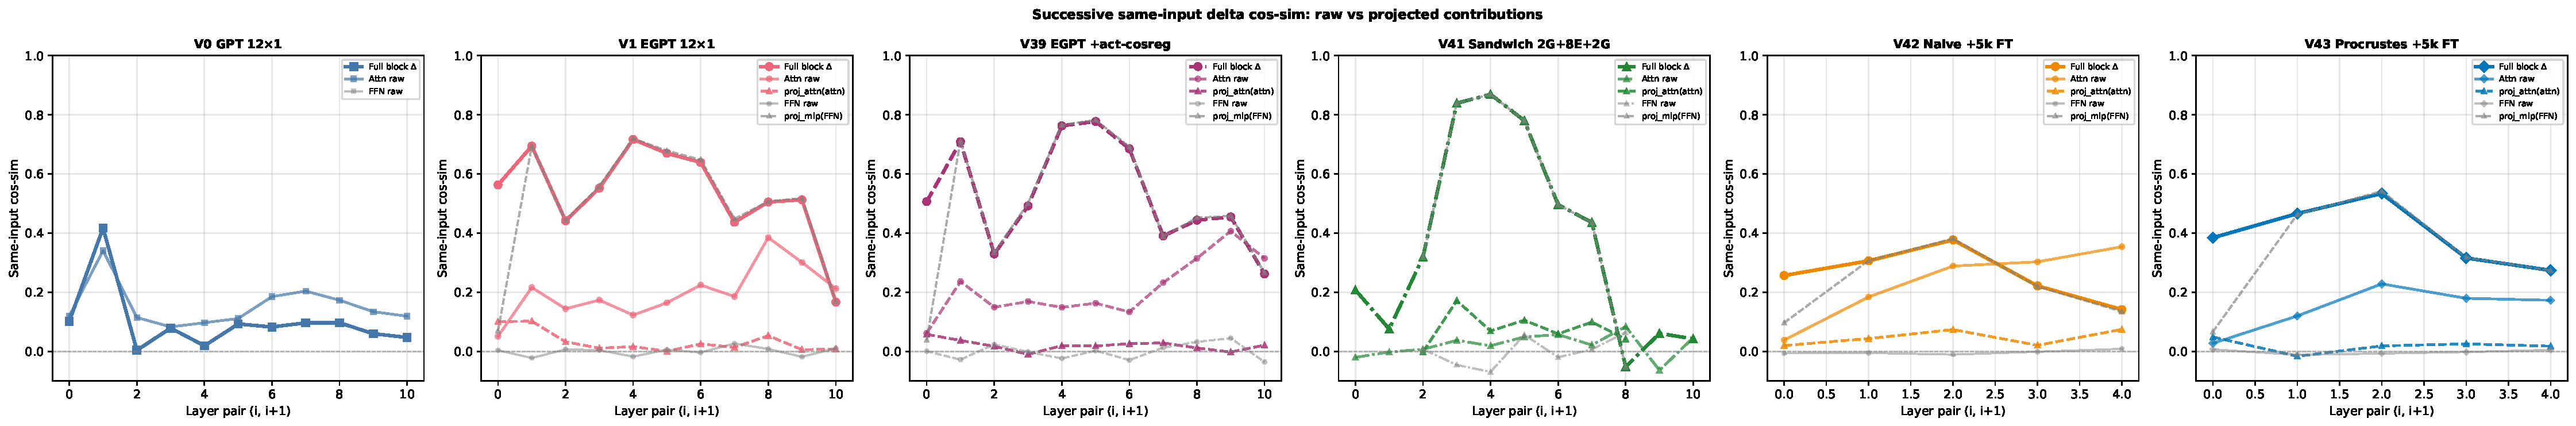
\includegraphics[width=\textwidth]{../results/multi-block-ablation/plots/proj_decomp_successive.pdf}
\caption{Successive same-input delta cosine similarity decomposed into raw vs.\ projected contributions.
  ``Attn raw'' = $\cos(a_i, a_{i+1})$;
  ``proj\_attn(attn)'' = $\cos(\mathrm{proj\_attn}_i(a_i), \mathrm{proj\_attn}_{i+1}(a_{i+1}))$;
  ``FFN raw'' / ``proj\_mlp(FFN)'' similarly.
  Shows whether the projection layer amplifies or creates inter-block alignment.}
\label{fig:proj_decomp_successive}
\end{figure}

\begin{figure}[h]
\centering
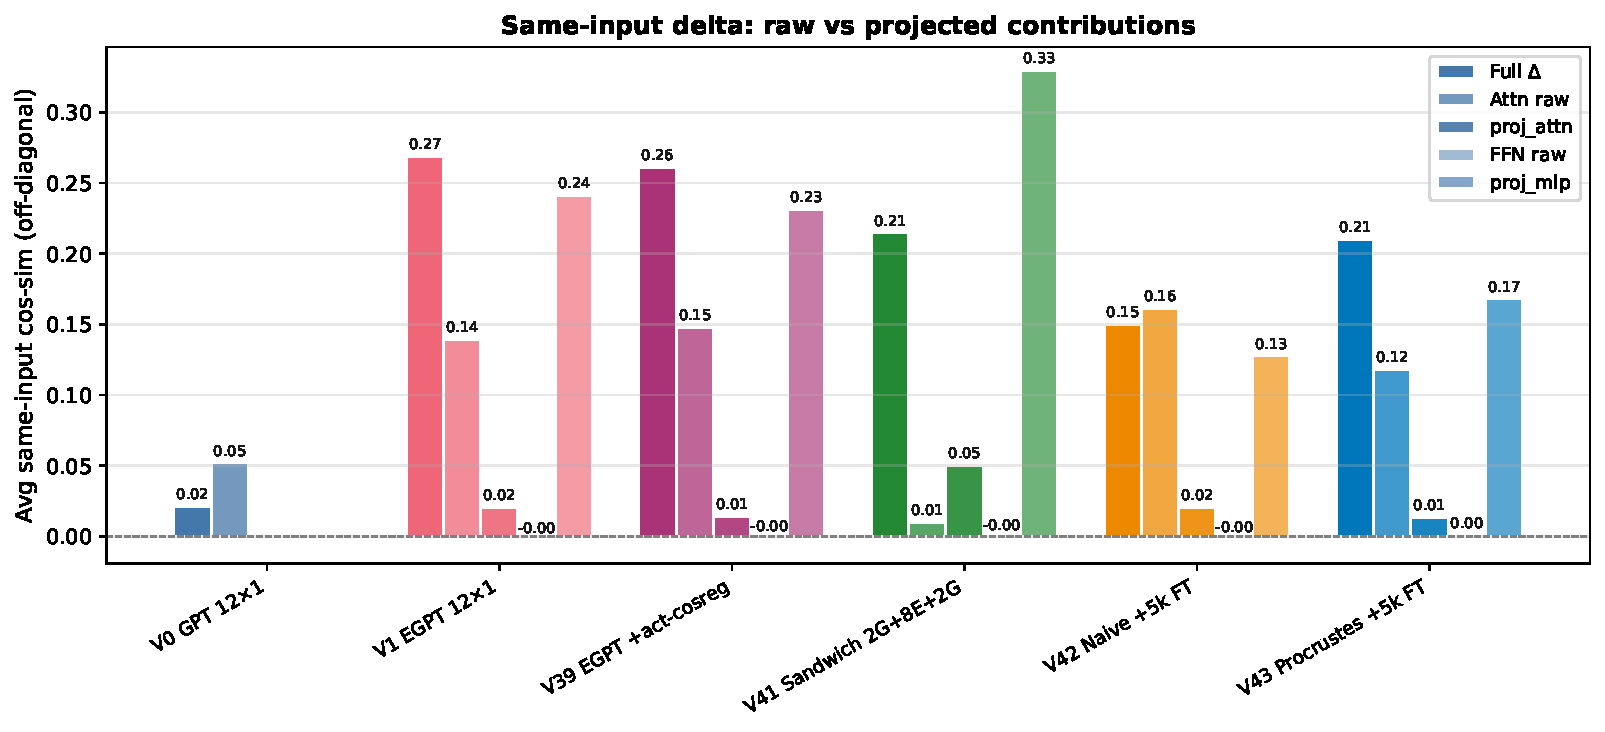
\includegraphics[width=\textwidth]{../results/multi-block-ablation/plots/proj_decomp_bar.pdf}
\caption{Off-diagonal mean: raw vs.\ projected same-input delta cosine similarity per model.}
\label{fig:proj_decomp_bar}
\end{figure}

\begin{figure}[h]
\centering
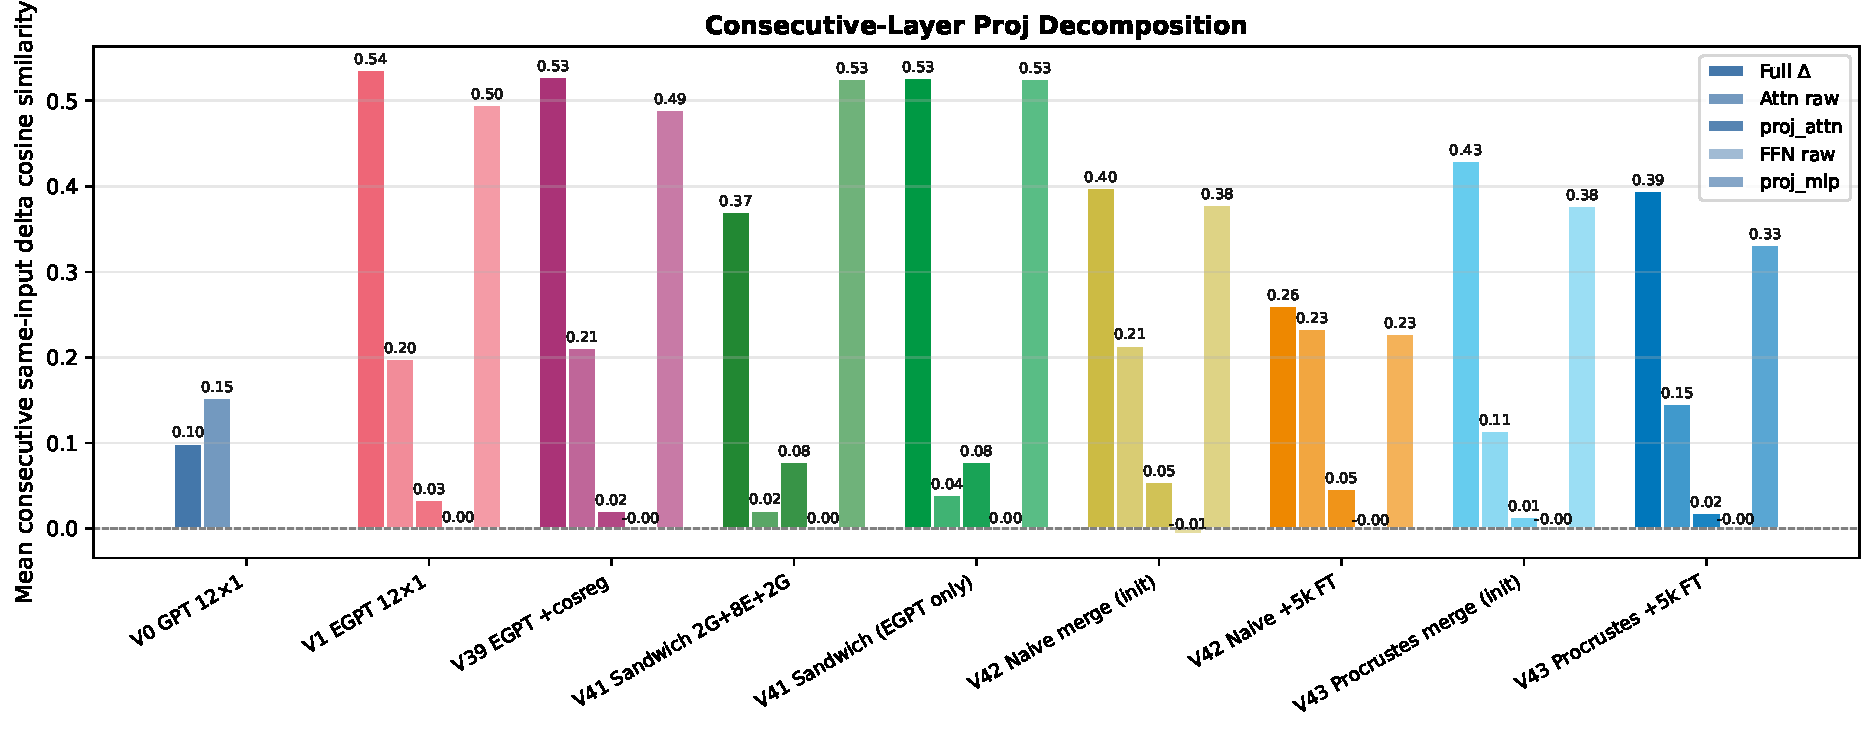
\includegraphics[width=\textwidth]{../results/multi-block-ablation/plots/proj_decomp_consec_bar.pdf}
\caption{Consecutive-layer mean: raw vs.\ projected same-input delta cosine similarity per model.
  V41 EGPT-only shows the projection decomposition restricted to EGPT-EGPT adjacent pairs.}
\label{fig:proj_decomp_consec_bar}
\end{figure}

%% -----------------------------------
\subsection{Strategy C: Sandwich Architecture (GPT Encoder + EGPT Core + GPT Decoder)}
\label{sec:sandwich}
%% -----------------------------------

\paragraph{Motivation.}
The full-layer cosine-similarity analysis (\S\ref{sec:probes}) shows a consistent pattern:
\emph{the first and last EGPT layers are least similar to their neighbours},
while the middle layers form a high-similarity cluster.  This suggests the boundary layers
serve a qualitatively different role --- adapting the input representation to the energy
manifold (layer 0) and projecting back out (layer 11).

We hypothesise that replacing these boundary layers with standard GPT
(softmax-attention + residual MLP) layers could provide a cleaner interface for the EGPT
core, potentially improving both raw performance and post-training mergeability of the
inner layers.

\paragraph{Architecture.}
\textbf{V41}: 2 standard GPT layers (softmax\_attention + MLP, additive residual) $+$ 8
EGPT layers (energy\_attention + Energy\_MLP, subtractive energy descent) $+$ 2 standard GPT
layers.  Total 12 layers, $d{=}768$, $\sim$176M parameters --- iso-param to V1.

\paragraph{Expected outcomes.}
\begin{enumerate}
  \item Lower PPL than V1 (boundary layers are easier for GPT; EGPT core trains with
        better-conditioned inputs / residuals).
  \item Higher cosine similarity among the 8 inner EGPT layers than the V1 inner layers.
  \item Post-merge of the 8 inner EGPT layers should be easier than V1 full-model merge.
\end{enumerate}

\paragraph{Results.}
V41 trained to 30k steps (loss 3.403 at 15k; full 30k results pending).
Activation-space analysis (Apr 25, 2026) shows the inner EGPT layers have
high mutual similarity (successive mean for layers 2--9: $\approx$0.983),
but the GPT$\leftrightarrow$EGPT boundaries are dramatically different:
layer 1$\to$2 (GPT$\to$EGPT): 0.977; layer 9$\to$10 (EGPT$\to$GPT): 0.729;
layer 10$\to$11 (last GPT boundary): 0.368.
The final boundary is the most disruptive, consistent with the output GPT layers
serving as a projection-back step that applies a large transformation.
This suggests sandwich architecture boundary layers are \emph{not} good merge candidates
despite the high inner-layer similarity.

\subsection{Summary}

\begin{table}[h]
\centering
\caption{Layer merger experiments.  ActSim = activation-space consecutive cosine similarity
  (successive mean).  Loss values are train CE loss.  V44/V45 are iso-compute (6$\times$2).}
\label{tab:layer_merger}
\resizebox{\textwidth}{!}{%
\begin{tabular}{lrrrrrl}
\toprule
\textbf{Model} & \textbf{Arch} & \textbf{Params} & \textbf{Loss} & \textbf{ActSim (init)} & \textbf{ActSim (FT)} & \textbf{Notes} \\
\midrule
V1  EGPT reference     & 12$\times$1 & 176M & 3.271 & 0.939 & --- & baseline \\
V39 CosReg 160M        & 12$\times$1 & 176M & 3.273 & 0.922 & --- & $\lambda{=}0.01$ cosreg \\
V41 Sandwich 2+8+2     & 12$\times$1 & 176M & 3.403 & 0.889 & --- & GPT+EGPT+GPT \\
\midrule
V42 Naive merge        &  6$\times$1 &  96M & 3.691 & 0.644 & 0.855 & half compute \\
V43 Procrustes merge   &  6$\times$1 &  96M & 3.640 & 0.756 & 0.853 & half compute \\
\midrule
V44 Naive 6$\times$2   &  6$\times$2 & 176M & 3.606 & 0.644 & --- & iso-compute \\
V45 Procrustes 6$\times$2 & 6$\times$2 & 176M & 3.584 & 0.756 & --- & iso-compute \\
\midrule
V46 Procrustes, const $lr{=}2\mathrm{e}{-}4$ & 6$\times$2 & 176M & 3.560 & 0.756 & --- & 5k FT \\
V47 Procrustes, cosine $2\mathrm{e}{-}3{\to}2\mathrm{e}{-}4$ & 6$\times$2 & 176M & \textbf{3.464} & 0.756 & --- & 5k FT \\
V49 Procrustes, const $lr{=}2\mathrm{e}{-}3$ & 6$\times$2 & 176M & 3.650 & 0.756 & --- & 5k FT; too noisy \\
V51 Procrustes, cosine $2\mathrm{e}{-}3{\to}2\mathrm{e}{-}4$ & 6$\times$2 & 176M & --- & 0.756 & --- & 10k FT; running \\
\bottomrule
\end{tabular}}
\end{table}

%% ============================================================
